\documentclass[12pt]{article}
\usepackage[portuguese, brazilian, english]{babel}
\usepackage[utf8]{inputenc}
\usepackage[usenames,dvipsnames]{color}
\usepackage{setspace}
\usepackage{amsmath}
\usepackage{amsfonts}
\usepackage{amssymb}
\usepackage{mathtools}
\usepackage[top=3cm, bottom=2cm, left=3cm, right=2cm]{geometry}
\usepackage{tikz}
\usepackage{textcomp}
\usepackage{lscape}    % for landscape pages
\usepackage{hyperref}  % to allow hyperlinks
\usepackage{booktabs}  % nicer table borders
\usepackage{subfigure} % add subfigures
\usepackage[bottom]{footmisc}

\title{Projeto de algoritmos baseados em florestas de posets
para o problema de otimização U-Curve}

% Figures directory
\graphicspath{{./figures/}} 

\definecolor{myblue}{RGB}{80,80,160}
\definecolor{mygreen}{RGB}{80,160,80}
\setstretch{1.5}



\setstretch{1.5}

\begin{document}
\selectlanguage{brazilian}
\thispagestyle{empty} 
\begin{flushright}
    {\LARGE Projeto de algoritmos baseados em florestas de posets\\
        \bigskip 
        para o problema de otimização U-curve \footnote{Uma versão
        muito parecida deste texto foi utilizada como uma proposta de
        iniciação científica, enviada à FAPESP, e outorgada como 
        processo de número 2016/25959-7. Aluno e orientador são os 
        mesmos do processo.}}


  \bigskip
  \bigskip
        
  {\large {\bf Aluno:} \href{mailto:gustavo.estrela.matos@usp.br}
        {Gustavo Estrela de Matos}\\ 
  {\bf Orientador:} \href{mailto:marcelo.reis@butantan.gov.br}
        {Marcelo da Silva Reis}\\
  \bigskip
  }

  \bigskip
  \bigskip
\end{flushright}

\begin{abstract}
% Resumo
O problema U-curve é uma formulação de um problema de otimização que
pode ser utilizado na etapa de seleção de características em Aprendizado
de Máquina, com aplicações em desenho de modelos computacionais de 
sistemas biológicos. Não obstante, soluções propostas até o presente 
momento para atacar esse problema têm limitações do ponto de vista de 
consumo de tempo computacional e/ou de memória, o que implica na 
necessidade do desenvolvimento de novos algoritmos. Nesse sentido, em
2012 foi proposto o algoritmo Poset-Forest-Search ({\tt PFS}), que 
organiza o espaço de busca em florestas de posets. Esse algoritmo foi 
implementado e testado, com resultados promissores; todavia, novos 
melhoramentos são necessários para que o {\tt PFS} se torne uma 
alternativa competitiva para resolver o problema U-curve. Neste 
projeto propomos a construção de uma versão paralelizada e escalável 
do algoritmo {\tt PFS}, utilizando diagramas de decisão binária 
reduzidos e ordenados. Além disso, propomos adaptar o {\tt PFS} como 
um algoritmo de aproximação, no qual o critério de aproximação da 
solução ótima faça uso do teorema da navalha de Ockham. Os algoritmos 
desenvolvidos serão implementados e testados em instâncias artificiais 
e também em conjuntos de dados próprios para experimentos comparativos 
entre diferentes algoritmos de seleção de características.
\end{abstract}



\section{Introdução}
% Apresentação do problema U-curve (na linha do projeto da primeira IC,
% só que procurando ser mais sucinto);
% Recapitulação da IC anterior (melhoramentos do algoritmo UCS com 
% ROBDDs), com particular destaque para a limitação dos melhoramentos 
% obtidos.
% 
\subsection{O problema U-curve}
O problema de seleção de característica consiste em, dado um conjunto $S$
de características, escolher um subconjunto de $S$ que seja
ótimo de acordo com
alguma métrica. A solução desse problema tem aplicações em
Aprendizado de Máquina e Reconhecimento de Padrões, com aplicações práticas
em identificação de sistemas biológicos -- por exemplo, na estimação de redes
gênicas regulatórias. Formalmente, podemos 
definir o problema de seleção de características como um problema de 
busca, no qual procuramos por um subconjunto $X \in \mathcal{P}(S)$ que 
minimiza uma função de custo $c : \mathcal{P}(S) \to \mathbb{R^+}$.
O espaço de busca do problema de seleção de características pode ser
estruturado como um reticulado Booleano ($\mathcal{P}(S)$, $\subseteq$), no qual
cada elemento é um subconjunto de características. Em funções custo $c$ que dependem
da estimação de uma distribuição conjunta a partir de um número limitado de
amostras, é comum que o custo das cadeias do reticulado, quando restritas a $c$,
descrevam curvas em U (figura~\ref{fig:U-curve}); esse
comportamento pode ser intuitivamente explicado se considerarmos que o
erro de estimação diminui ao adicionarmos novas características, até um ponto
em que a limitação de amostras faz com que acrescentar características
leve a um aumento no erro de estimação.

\begin{figure}[h]
\centering 
\begin{tabular}{c c}
    \subfigure[] {
        \scalebox{0.75}{
        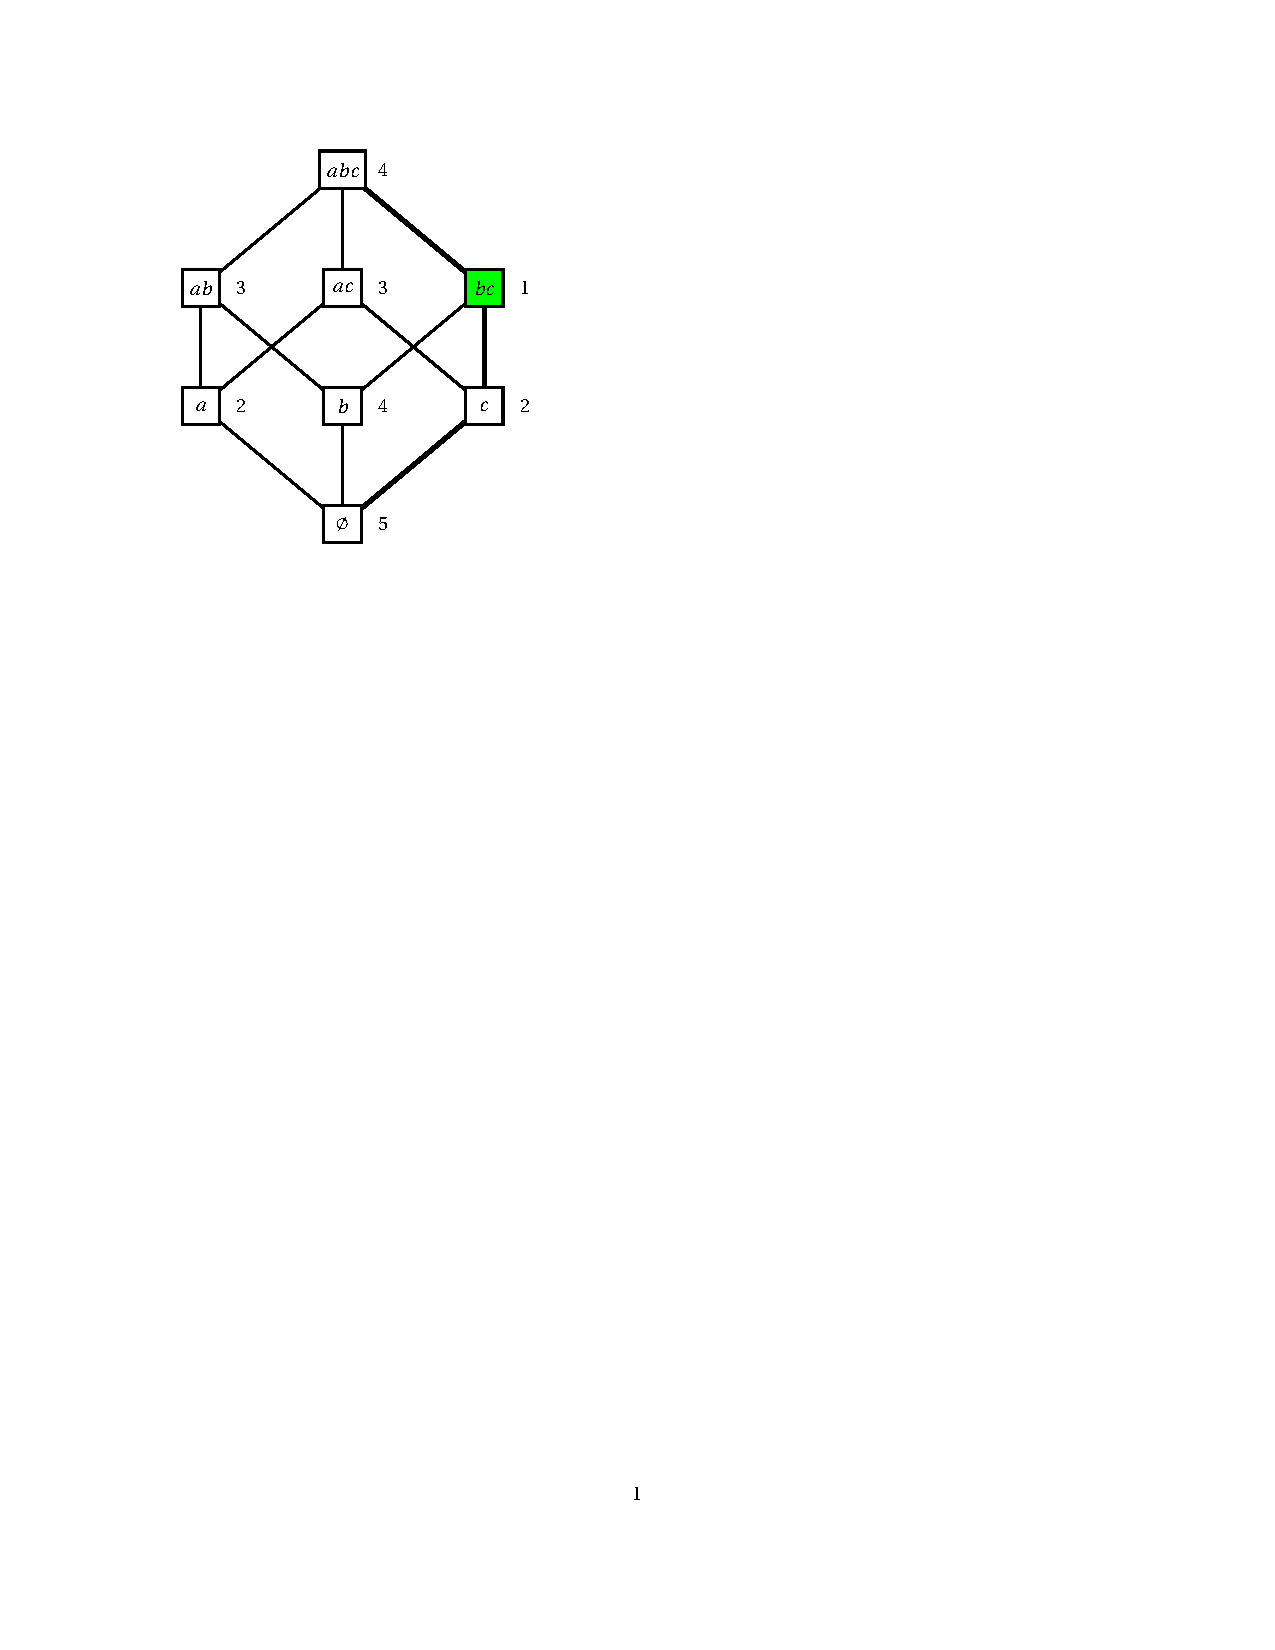
\includegraphics
        [trim=2cm 17.5cm 12.2cm 2cm,clip=true]{Boolean_lattice_3_A.pdf}}
        \label{fig:U-curve-example:A}
    }  
    &
    \subfigure[] {
        \scalebox{0.30}{
        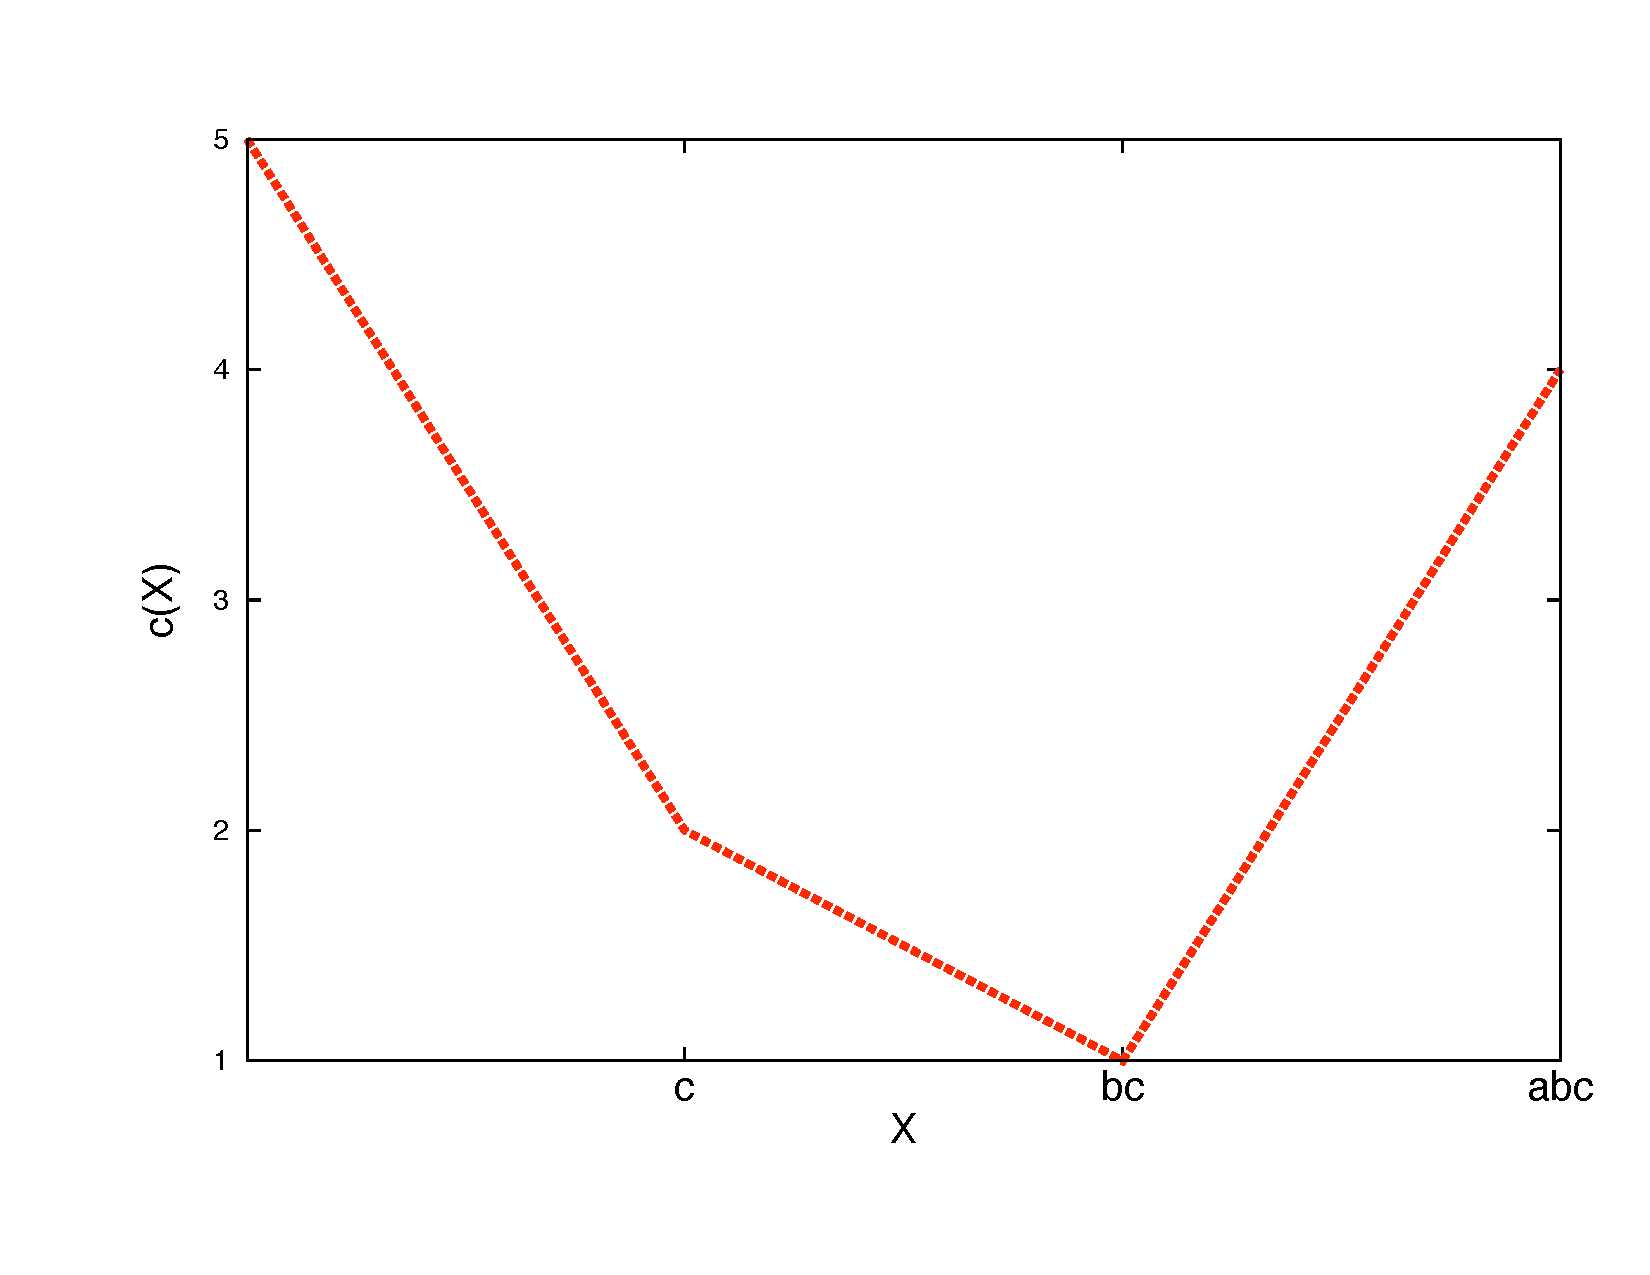
\includegraphics[clip=true]{exemplo1.pdf}} 
        \label{fig:U-curve-example:B} 
    }
\end{tabular}
\caption{exemplo de instância do problema U-curve. 
Figura~\ref{fig:U-curve-example:A}: o diagrama de Hasse de um reticulado
Booleano de grau $3$ -- as cadeias do reticulado, cujos custos de seus
elementos são definidos através dos números ao lado dos elementos, descrevem
curvas em U; a cadeia maximal $\{ \emptyset, c, bc, abc \}$ está
destacada em negrito. O elemento $bc$, destacado em verde, é mínimo na
cadeia (e também no reticulado Booleano). 
Figura~\ref{fig:U-curve-example:B}: o gráfico dos custos em função dos
elementos da cadeia maximal destacada em negrito, mostrando sua curva em
U. Figuras extraídas de Reis~\cite{msreis thesis}.} 
    \label{fig:U-curve} 
\end{figure}



O problema U-curve é um caso particular do problema de seleção de
características no qual todas as cadeias do espaço de busca descrevem
curvas em U quando avaliadas pela função de custo (figura~\ref{fig:U-curve}).
Existem algoritmos
ótimos para solução do problema U-curve, tais como o U-curve-Branch-and-Bound
({\tt UBB}) e o Poset-Forest-Search ({\tt PFS})~\cite{msreis thesis}; os
princípios de funcionamento deste último serão apresentados a seguir.


\subsection{O algoritmo Poset-Forest-Search ({\tt PFS})}
O algoritmo {\tt PFS} é um algoritmo ótimo do tipo 
{\em branch-and-bound}. A ideia básica é generalizar o algoritmo {\tt UBB},
que é um {\em branch and bound} unidirecional, em um procedimento bidirecional.
Para esse fim, {\tt PFS} inicializa representando o espaço de 
busca com duas árvores $T$ e $T'$ tais que $T'$ é uma árvore complementar a 
$T$, ou seja, para qualquer aresta $\{ X, Y \}$ na
árvore $T$ existe uma aresta $\{ X^c, Y^c \}$ na árvore $T'$ 
(figuras~\ref{fig:PFS_tree:A} e \ref{fig:PFS_tree:B}).


\begin{figure}[h]
  \centering 
  \begin{tabular}{c c}
    \subfigure[] {\scalebox{0.45}{
     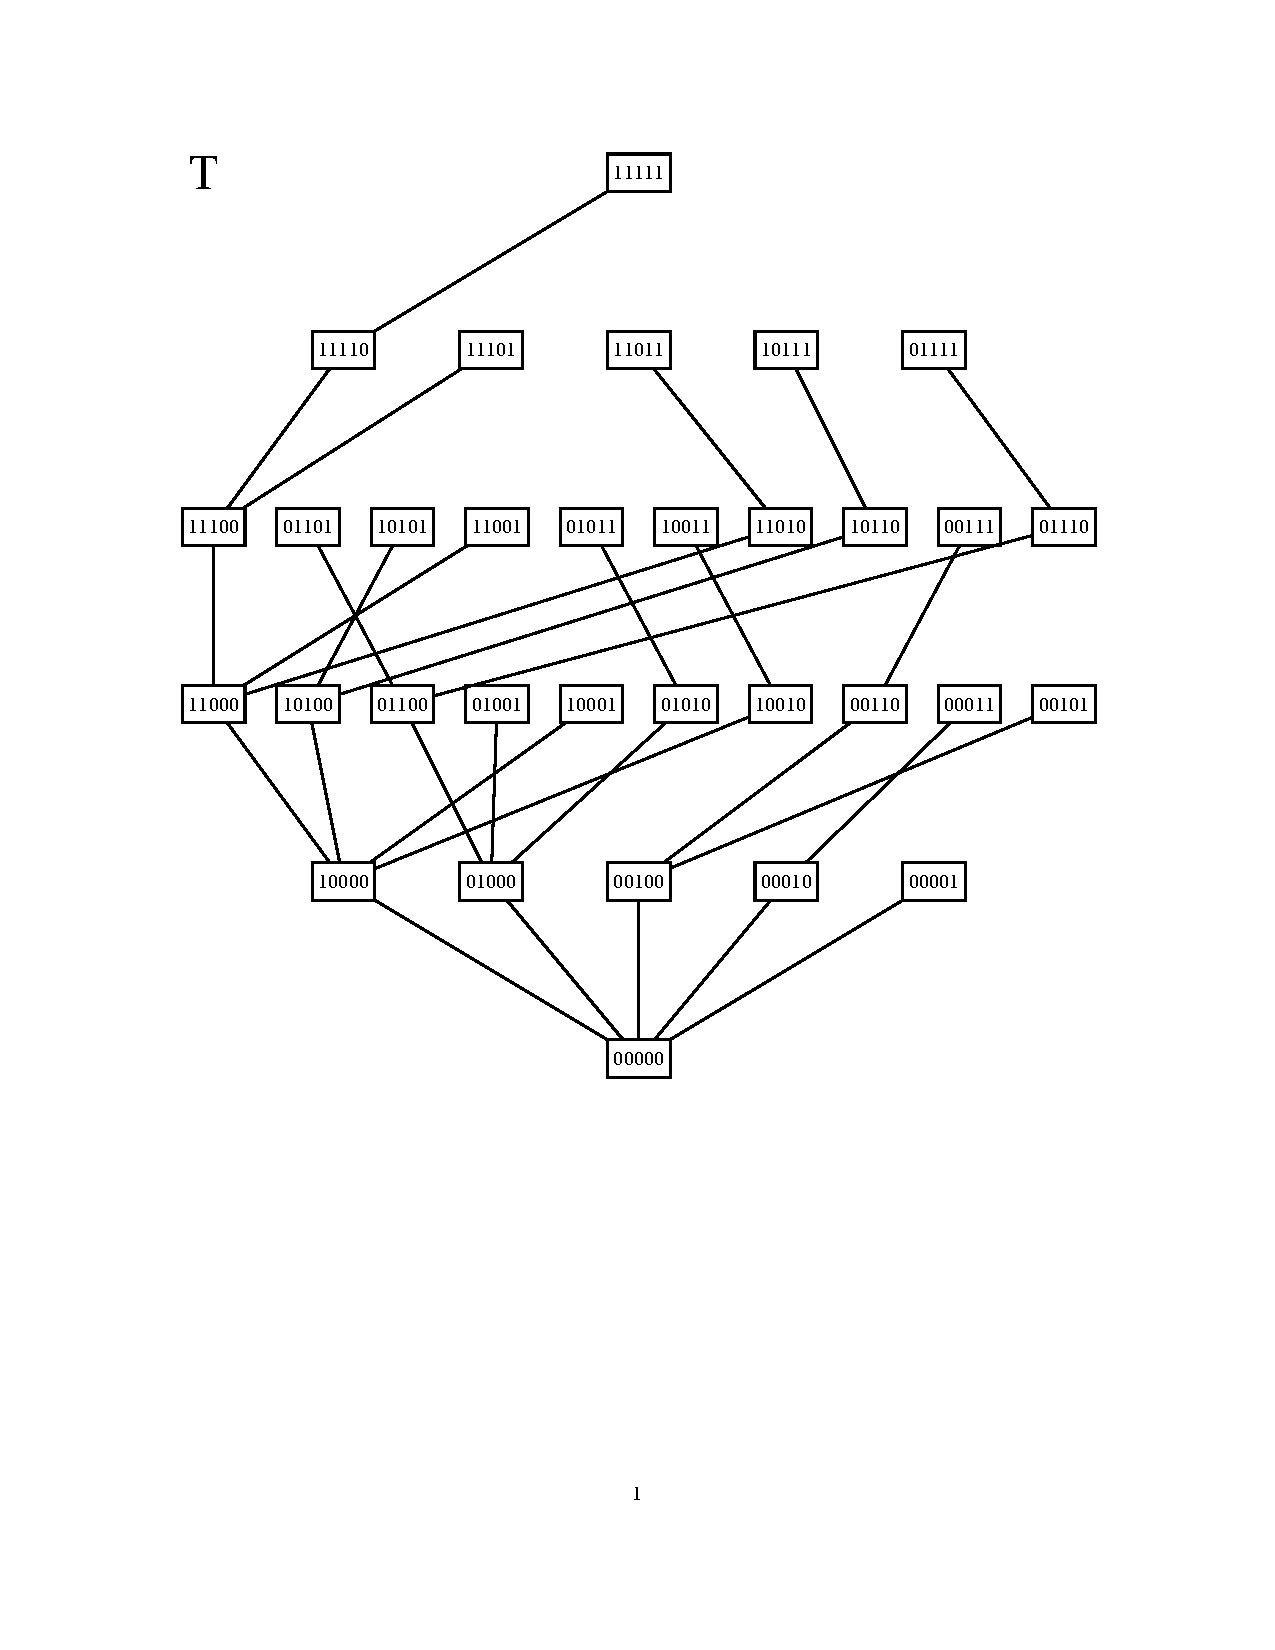
\includegraphics[trim=3cm 8.5cm 1.2cm 2cm, clip=true]{PFS_tree_A.pdf}}
     \label{fig:PFS_tree:A} }
    &
    \subfigure[] {\scalebox{0.45}{
    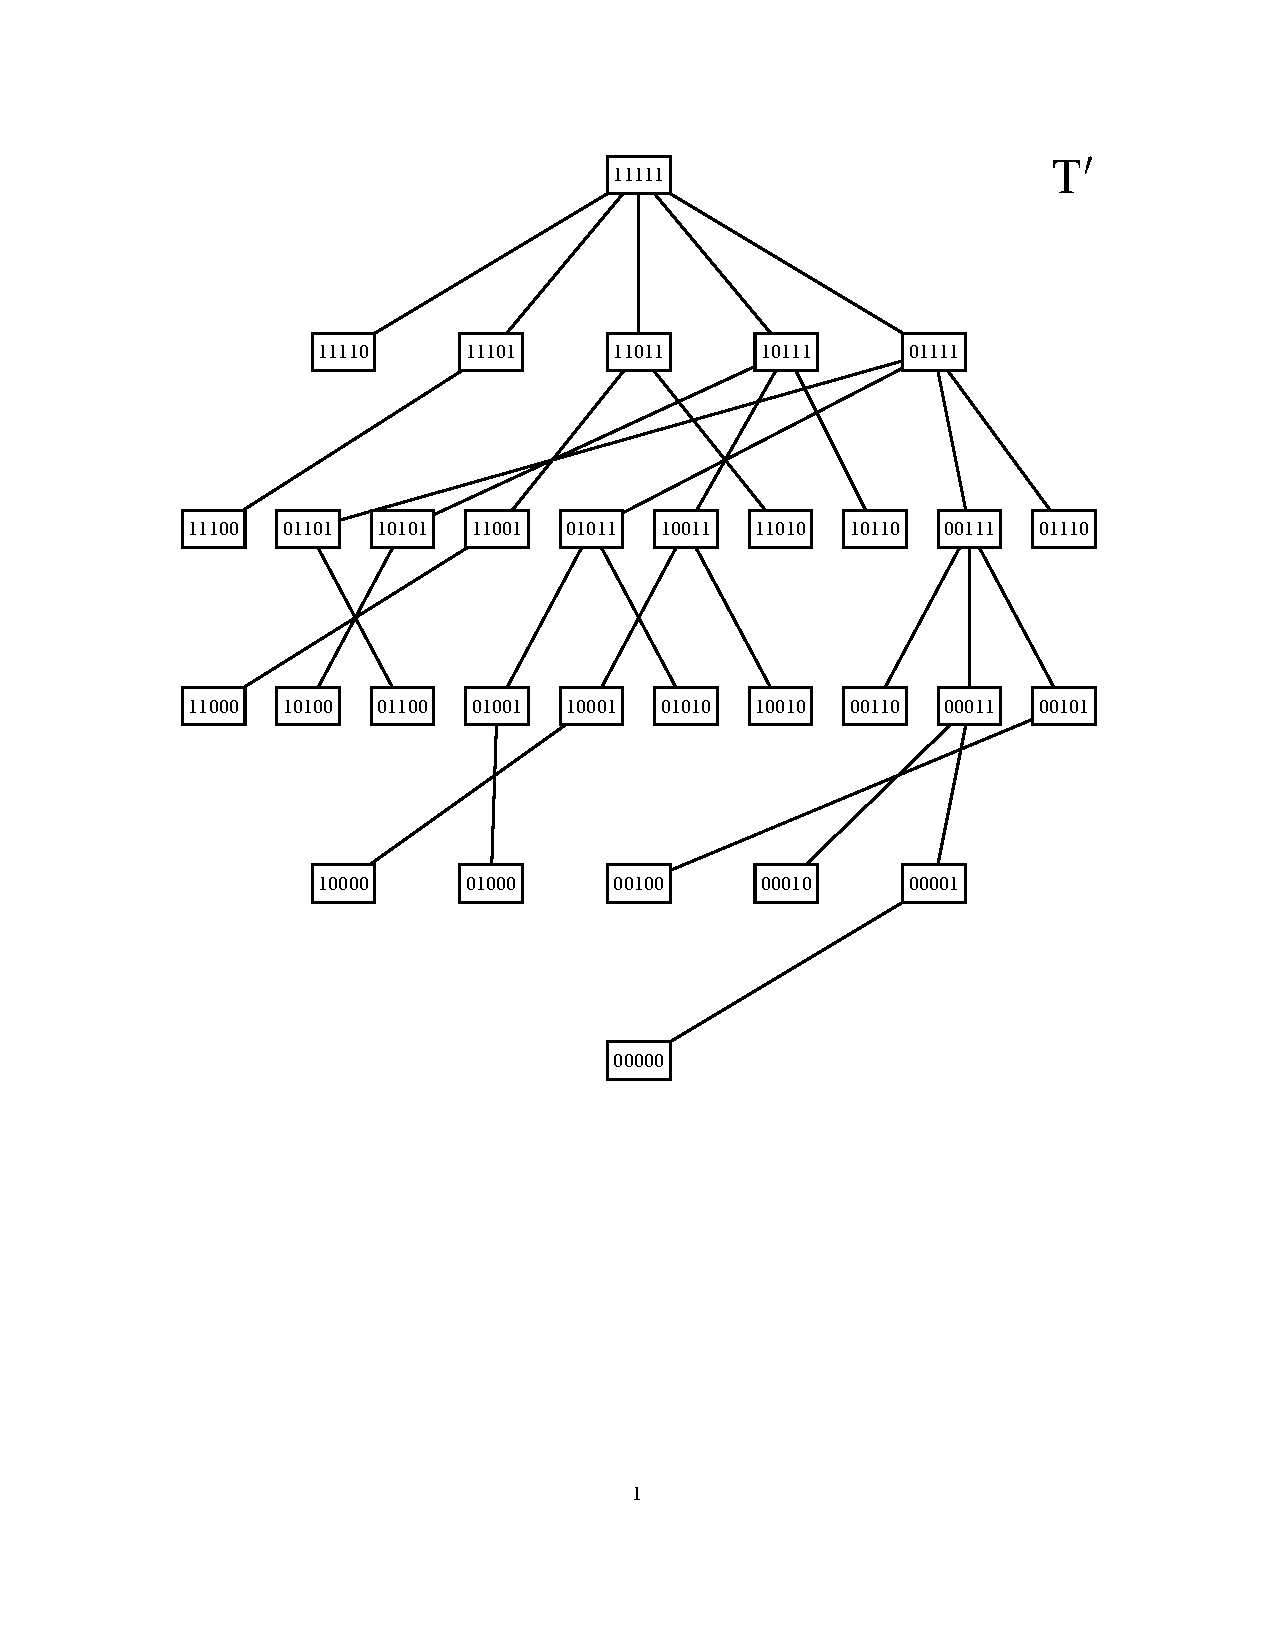
\includegraphics[trim=3cm 8.5cm 1.2cm 2cm, clip=true]{PFS_tree_B.pdf}}
    \label{fig:PFS_tree:B} }
  \end{tabular}
  \caption{exemplo de enumerações de um reticulado Booleano, no qual a
árvore $T$ (figura~\ref{fig:PFS_tree:A}) é complementar à árvore $T'$
(figura~\ref{fig:PFS_tree:B}). Figuras extraídas de Reis~\cite{msreis thesis}.}
  \label{fig:PFS_tree} 
\end{figure}

O algoritmo se inicializa escolhendo uma das duas árvores; sem perda de generalidade, digamos que $T$ foi escolhida. A partir
do conjunto vazio, uma cadeia é percorrida até que o custo de um elemento seja maior que o do elemento $X$ que o precedeu na cadeia (figura~\ref{fig:PFS_pruning:A}); nesse caso, são eliminados do espaço de busca todos os elementos que se ramificam na árvore $T$ a partir de $X$, assim como as arestas percorridas desde o conjunto vazio. Esse procedimento resulta em uma floresta $\mathcal{A}$ composta por três árvores (figura~\ref{fig:PFS_pruning:A}). Ao removermos de $T'$ os mesmos elementos que foram removidos de $T$, o grafo induzido pelas arestas remanescentes resulta em uma floresta $\mathcal{B}$ também composta por três árvores (figura~\ref{fig:PFS_pruning:B}).

O algoritmo {\tt PFS} inicia então uma nova iteração, escolhendo uma das florestas e em seguida repetindo o procedimento descrito acima para uma das árvores que a compõem. Se uma árvore é composta por um único elemento $X$ (i.e., uma árvore trivial, composta apenas por uma raiz), então $X$ é removido da floresta escolhida, e a outra floresta é atualizada eliminando-se $X$ e as arestas com uma das pontas ligada a esse elemento. O algoritmo {\tt PFS} itera até que todo o espaço de busca seja esgotado.


\begin{figure}[h]
  \centering 
  \begin{tabular}{c c}
    \subfigure[] {\scalebox{0.45}{
    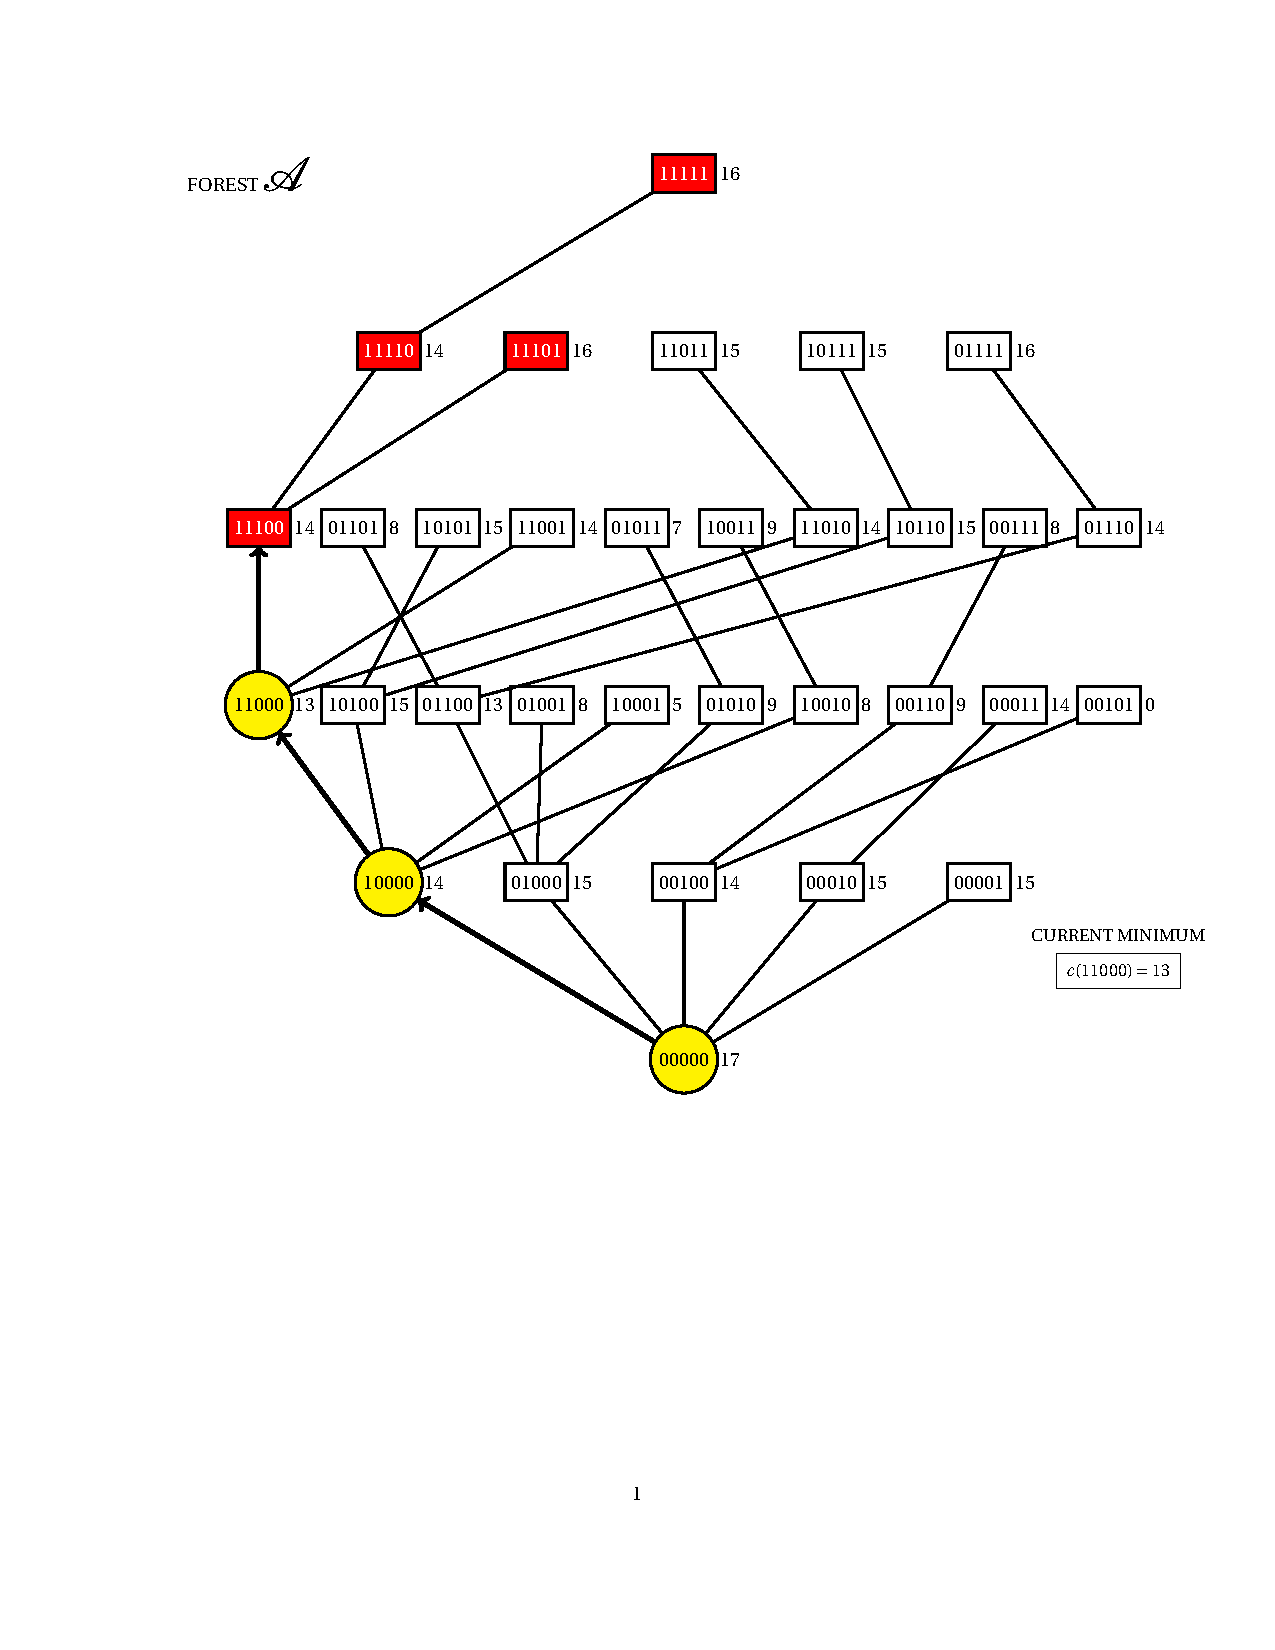
\includegraphics[trim=3cm 8.5cm 1.2cm 2cm, clip=true]{PFS_dynamics_D.pdf}}
    \label{fig:PFS_pruning:A}  }
    &
    \subfigure[] {\scalebox{0.45}{
    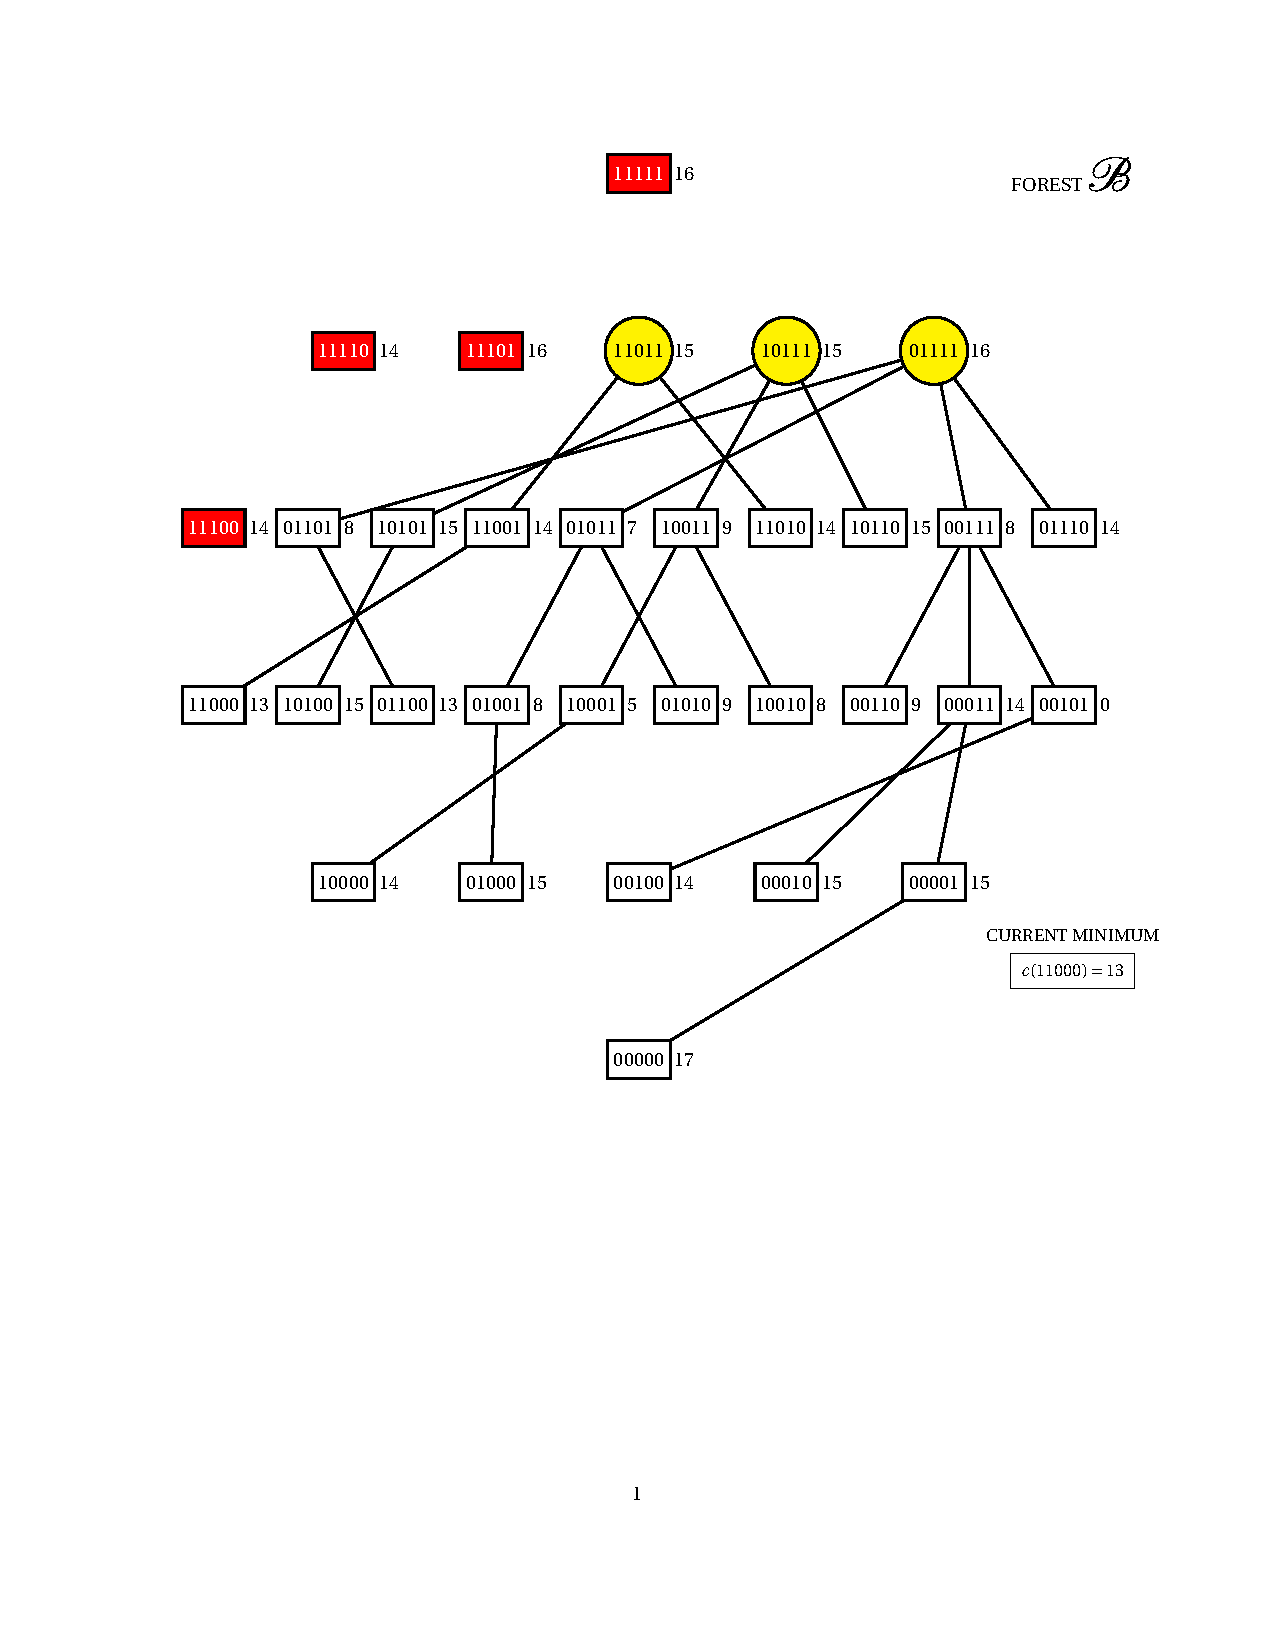
\includegraphics[trim=3cm 8.5cm 1.2cm 2cm, clip=true]{PFS_dynamics_G.pdf}}
    \label{fig:PFS_pruning:B}  }
  \end{tabular}
  \caption{exemplo de um percorrimento e poda realizados na árvore $T$, no qual é eliminado 
do espaço de busca o intervalo $[11100, 11111]$ e produzida uma floresta $\mathcal{A}$ contendo três árvores, cujas raízes estão destacadas em amarelo
(figura~\ref{fig:PFS_pruning:A}). A eliminação desse intervalo em $T'$ produz
uma floresta $\mathcal{B}$ também com três árvores (figura \ref{fig:PFS_pruning:B}). Figuras extraídas
de Reis~\cite{msreis thesis}.}
  \label{fig:PFS_pruning} 
\end{figure}

Uma versão preliminar do {\tt PFS} já foi implementada e mostrou resultados promissores, principalmente
quando analisado o número de elementos do reticulado que são visitados~\cite{msreis thesis}. Apesar
disso, o algoritmo apresenta propriedades interessantes que foram pouco exploradas nesse trabalho original; por exemplo, o gerenciamento do espaço de busca através de florestas poderia ser aproveitado para o desenvolvimento de algoritmos paralelizados ótimos para o problema U-curve, com maior escalabilidade em relação a variantes sequenciais. Ademais, seria interessante testar a aplicabilidade desse algoritmo em um conjunto abrangente de instâncias de interesse prático.




\section{Objetivos}
Neste trabalho, propomos atingir três objetivos:

\begin{enumerate}
\item Implementação de uma versão do algoritmo sequencial do algoritmo 
{\tt PFS} utilizando diagramas de decisão binária reduzidos e ordenados
{\em Reduced Ordered Binary Decision Diagrams} -- ROBDDs) para 
representar as listas de raízes da floresta que representa o espaço de
busca no algoritmo {\tt PFS}. ROBDD é uma estrutura de dados eficiente 
para gerenciar coleções de elementos de um reticulado 
Booleano~\cite{bryant}.

\item Desenho de uma versão escalável do {\tt PFS}. Para este fim, 
paralelizaremos o percorrimento das árvores nas florestas que 
representam o espaço de busca, com o programa principal gerenciando a 
escolha das raízes (i.e., início de um percorrimento), guardando o 
mínimo corrente e centralizando a atualização das podas.

\item Desenvolvimento de uma versão do {\tt PFS} que funcione como algoritmo 
de aproximação para o problema U-curve, utilizando como critério de
aproximação da solução ótima o teorema da navalha de Ockham:\\
\smallskip
Dado um espaço de hipóteses $H$ (i.e., espaço de busca), o número mínimo 
de amostras necessário para se obter uma solução que erra no máximo 
$\epsilon$ com $1 - \delta$ de probabilidade é expresso por:
\begin{equation}
\displaystyle  m(\delta,\epsilon) \ge 
    \frac{1}{\epsilon} log (\frac{|H|}{\delta}). \label{eq:Ockham}
\end{equation}
Este resultado da equação~\ref{eq:Ockham}, que é bem conhecido em teoria
de Aprendizado de Máquina~\cite{kearns}, será aproveitado para o uso das
variantes do algoritmo {\tt PFS} para resolver de forma aproximada 
instâncias de tamanho proibitivo mesmo para versões escaláveis do
algoritmo ótimo.
\end{enumerate}

Para todos os algoritmos propostos, faremos implementação e testes 
empíricos, para isso utilizando tanto instâncias artificiais quanto 
conjuntos de dados próprios para {\em benchmarking} de algoritmos de 
seleção de características.


\section{Plano de trabalho}
A pesquisa se iniciará com o estudo do algoritmo {\tt PFS}. Uma 
implementação desse algoritmo atualmente encontra-se disponível para o  
\href{https://github.com/msreis/featsel}{featsel}, e será 
usado como base para os futuros algoritmos deste projeto. O próximo 
passo envolverá a construção de uma modificação do algoritmo {\tt PFS}
que utiliza a estrutura de dados ROBDD para guardar as raízes da 
floresta que representa o espaço de busca do problema.

Em seguida, vamos analisar a dinâmica do algoritmo {\tt PFS} e
reescrevê-la com as necessárias modificações para que partes do
algoritmo possam ser executadas em paralelo. A princípio, a
paralelização do algoritmo se dará no percorrimento de caminhos das
florestas do espaço de busca, que será atualizado em um espaço comum da
memória a todas as linhas de execução. Ao final dessa etapa, teremos um
novo algoritmo, que será testado e comparado com outros algoritmos do
arcabouço featsel, tais como o {\tt UBB} e o {\tt PFS} original.

A próxima etapa do nosso trabalho será o estudo de algoritmos de 
aproximação e do \textit{Probably Approximately
Correct} (PAC learning), que é modelo de aprendizado no qual se aplica o
teorema da navalha de Ockham. Com isso, pretendemos construir uma 
variante do algoritmo {\tt PFS} que deixa de buscar uma solução ótima 
para buscar uma solução provavelmente aproximadamente correta. Após 
implementarmos o algoritmo de aproximação para o problema U-Curve 
poderemos testar o seu desempenho de forma análoga ao que será feito 
com a versão paralelizada com OpenMP.

Depois, testaremos todos os algoritmos desenvolvidos durante o projeto
com instâncias artificiais e reais do problema U-Curve. Para gerar 
instâncias artificiais, empregaremos a redução polinomial do problema 
{\em subset sum} para instâncias do problema U-curve apresentada em 
Reis~\cite{msreis thesis}, assim como outras funções custo  nas quais
são introduzidas oscilações nas curvas em U das cadeias
do reticulado Booleano. Já para instâncias reais, utilizaremos conjuntos
de dados próprios para benchmarking de algoritmos, tais como os 
abrigados no \href{archive.ics.uci.edu/ml}{UCI Machine Learning 
Repository}.

Durante os seis últimos meses de trabalho pretendemos escrever a 
monografia, que deverá conter uma explicação detalhada do problema 
que abordamos, o desenvolvimento do trabalho e também dados e análise
dos resultados obtidos. Concluída essa etapa, uma versão reduzida desse
texto deverá compor a apresentação e pôster desse trabalho.

Um cronograma para este projeto proposto é apresentado na 
tabela~\ref{tab:cronograma}, enquanto que o detalhamento das atividades
listadas no mesmo é feito na seção~\ref{sec:atividades}.

\subsection{Cronograma}
\begin{table}[!ht]
\caption{cronograma de atividades previstas nesta proposta de projeto.} 
\label{tab:cronograma}
\begin{center}
\smallskip
\begin{tabular}{l cccccccc}
    \toprule
    \small Atividade/mês & \small Mai.17 & \small Jun.17 & \small Jul.17
                         & \small Ago.17 & \small Set.17 & \small Out.17
                         & \small Nov.17 & \small Dez.17
    \\ \hline

    \small Atividade 1   
    & \small {\bf x} & \small - & \small - & \small - & \small -
    & \small - & \small - & \small - \\
    

    \small Atividade 2   
    & \small {\bf x} & \small - & \small - & \small - & \small -
    & \small - & \small - & \small - \\

    \small Atividade 3   
    & \small - & \small {\bf x} & \small {\bf x} & \small - & \small -
    & \small - & \small - & \small - \\

    \small Atividade 4
    & \small - & \small - & \small {\bf x} & \small {\bf x} & \small -
    & \small - & \small - & \small - \\

    \small Atividade 5   
    & \small - & \small - & \small {\bf x} & \small {\bf x} & \small -
    & \small - & \small - & \small - \\

    \small Atividade 6   
    & \small - & \small - & \small - & \small {\bf x} & \small {\bf x}
    & \small - & \small - & \small - \\

    \small Atividade 7
    & \small - & \small - & \small - & \small - & {\bf x}
    & \small {\bf x} & \small - & \small - \\

    \small Atividade 8  
    & \small - & \small - & \small - & \small - & -
    & \small {\bf x} & \small {\bf x} & \small {\bf x} \\

    \small Atividade 9
    & \small - & \small - & \small - & \small - & \small -  
    & \small - & \small {\bf x} & \small - \\

    \small Atividade 10
    & \small - & \small - & \small - & \small - & \small -  
    & \small - & \small - & \small {\bf x} \\

    \small Atividade 11
    & \small - & \small - & \small {\bf x} & \small {\bf x} 
    & \small {\bf x}  & \small {\bf x} & \small {\bf x}
    & \small {\bf x} \\



    \bottomrule
\end{tabular}
\end{center}
\end{table}

\subsection{Descrição de atividades} \label{sec:atividades}
\begin{itemize}
    \item{\bf Atividade 1.}
        Estudo do algoritmo {\tt PFS}.
    \item{\bf Atividade 2.}
        Implementação de uma variante do {\tt PFS} que usa ROBDDs como 
        estrutura de dados para representar as coleções de raízes das 
        árvores das florestas.
    \item{\bf Atividade 3.}
        Implementação de uma versão paralela do algoritmo {\tt PFS} com
        o uso de ROBDDs como estrutura de dados.
    \item{\bf Atividade 4.}
        Testes da primeira versão do {\tt PFS} paralelizado com 
        instâncias artificiais.
    \item{\bf Atividade 5.}
        Estudos do {\em PAC learning} e do teorema da navalha de Ockham.
    \item{\bf Atividade 6.}
        Implementação de versões do {\tt PFS}, sequencial e 
        paralelizada, que se comportem como algoritmos de aproximação.
    \item{\bf Atividade 7.} 
        Testes com instâncias artificiais dos algoritmos de aproximação.
    \item{\bf Atividade 8.}
        Estudo comparativo entre os algoritmos produzidos, incluindo 
        testes com instâncias artificiais e também de problemas reais.
    \item{\bf Atividade 9.}
        Elaboração do pôster e apresentação.
    \item{\bf Atividade 10.}
        Escrita do relatório de iniciação científica
    \item{\bf Atividade 11.}
        Escrita da monografia.
    \end{itemize}

\subsection{Atividades realizadas}
Em um outro trabalho, onde criamos um algoritmo paralelo para o problema
U-Curve, tivemos a oportunidade de estudar e praticar o uso da 
biblioteca OpenMP. Além disso, em uma iniciação científica anterior 
~\cite{ucsrobdd ic}, implementamos a estrutura de dados ROBDD no mesmo
arcabouço que propomos usar neste trabalho.

% Arcabouço featsel, já contando com os acréscimos de classes de ROBDDs;
% Biblioteca OpenMP.
\section{Materiais e métodos}
Os algoritmos produzidos serão implementados no arcabouço 
\href{https://github.com/msreis/featsel}{featsel}. Esse arcabouço foi 
implementado em C++ e conta com diversas estruturas de dados que serão
necessárias para implementar os algoritmos sugeridos neste trabalho.
Além disso, featsel já conta com classes que implementam ROBDDs; tal
melhoramento foi feito durante a Iniciação Científica anterior do
aluno, numa tentativa de melhorar o desempenho do algoritmo
U-Curve-Search ({\tt UCS}), resultando em ganhos modestos de desempenho
do ponto de vista de desempenho computacional~\cite{ucsrobdd ic}.
O arcabouço featsel está disponível sob a licença \textit{GNU General
Public License} (GNU-GPL), o que nos permite utilizar livremente o
código desse arcabouço para implementação dos novos algoritmos. 

Também utilizaremos a biblioteca \href{http://www.openmp.org/}{OpenMP}
junto ao compilador {\tt g++} para compilar os códigos produzidos.
Por meio de diretivas de compilação, OpenMP determina como um código
pode ser executado em paralelo no processador.

Experimentos computacionais, em particular os que envolverem 
paralelização de algoritmos, serão feitos em uma servidora do Instituto
Butantan que é própria para esse fim: uma Dell PowerEdge 850, com 64 
núcleos e 256 GB de memória RAM.


% Benchmarking contra outros algoritmos de seleção de características;
% Elaboração de paper para ser enviado para publicação ao final da IC
% proposta.
\section{Forma de Análise e de Divulgação dos Resultados}

Para analisar os resultados obtidos utilizaremos o próprio arcabouço
\href{https://github.com/msreis/featsel}{featsel}, que já possui métodos
que registram dados sobre a execução dos algoritmos, assim como um
programa auxiliar para {\em benchmarking} de algoritmos e de funções
custo implementados nessa ferramenta. As principais métricas a serem 
consideradas nos experimentos serão tempo de execução, consumo de 
memória e a robustez dos algoritmos quando violamos a suposição de que 
a função custo é decomponível em curvas em U. O código-fonte final do 
projeto será disponibilizado para a comunidade acadêmica no 
\href{https://github.com/msreis/featsel}{repositório web do arcabouço
featsel}.

Os resultados obtidos e os conhecimentos adquiridos ao longo deste
projeto serão apresentados na forma de uma apresentação para colegas de
curso e professores; na forma de pôster, o qual será exposto no IME;
e também em uma monografia. Além disso, todo o desenvolvimento deste 
projeto deve ser reportado a FAPESP no formato de relatório de iniciação
científica.

Por fim, projetamos a escrita de um artigo científico, no qual 
descreveremos os avanços que os novos algoritmos trouxeram, além de
eventuais propriedades do problema U-Curve e de nossa solução que possam
ser exploradas futuramente para elaboração de novas abordagens para 
resolver esse importante problema de otimização.


\begin{thebibliography}{}
\addcontentsline{toc}{section}{Referências}
\bibitem{msreis thesis}
    Marcelo S. Reis. ``Minimização de funções decomponíveis em curvas em U definidas sobre cadeias de posets -- algoritmos e aplicações".
    Tese de doutorado. Instituto de Matemática e Estatística, Universidade de São Paulo, Brasil (2012).

\bibitem{bryant}
Randal E. Bryant. ``Graph-based algorithms for boolean function manipulation". IEEE Transactions on Computers, 100.8 (1986): 677-691. 

\bibitem{kearns}
Michael J. Kearns e Umesh V. Vazirani. ``An introduction to computational learning theory". MIT Press (1994).

\bibitem{ucsrobdd ic}
Gustavo E. Matos e Marcelo S. Reis. ``Estudos de estruturas de dados eficientes para abordar o problema de otimização U-curve". Relatório científico final FAPESP, Instituto Butantan, Brasil (2015).

\end{thebibliography}
\end{document}
